% % % % % % % % % % % % % % % % % % % % % % % % % % % % % % % % % % % % % % % % % % % %
%                                                                                     %
% Short Sectioned Assignment LaTeX Template Version 1.0 (5/5/12)                      %
% This template has been downloaded from: http://www.LaTeXTemplates.com               %
%                                                                                     %
% Original author:  Frits Wenneker (http://www.howtotex.com)                          %
%                                                                                     %
% Modified by: Fco Javier Sueza Rodríguez (fcosueza@disroot.org)                      %
%                                                                                     %
% Changes:                                                                            %
%	    - Custom Chapters, Sections and Subsections (titlesec package)                %
%           - Document type scrbook (oneside)                                         %
%           - Use babel-lang-spanish package and marvosym                             %
%           - Use hyperref, enumitem, tcolorbox and glossaries packages               %
%           - Use Time New Roman (mathptmx), Helvetic and Courier fonts               %
%                                                                                     %
% License: CC BY-NC-SA 3.0 (http://creativecommons.org/licenses/by-nc-sa/3.0/)        %
%                                                                                     %
% % % % % % % % % % % % % % % % % % % % % % % % % % % % % % % % % % % % % % % % % % % %

%-----------------------------------------------%
%	              Packages                  %
%-----------------------------------------------%

\documentclass[paper=a4, fontsize=11pt, oneside]{scrbook}

% ---- Text Input/Output ----- %

\usepackage[T1]{fontenc}
\usepackage[utf8]{inputenc}
\usepackage{mathptmx}
\usepackage[scaled=.92]{helvet}
\usepackage{courier}
\usepackage[indent=12pt]{parskip}

\usepackage{geometry}
\geometry{verbose,tmargin=3cm,bmargin=3cm,lmargin=2.6cm,rmargin=2.6cm}

% ---- Language ----- %

\usepackage[spanish]{babel}
\usepackage{marvosym}

% ---- Another packages ---- %

\usepackage{amsmath,amsfonts,amsthm}
\usepackage{graphics,graphicx}
\usepackage{titlesec}
\usepackage{fancyhdr}
\usepackage{tcolorbox}
\usepackage{hyperref}
\usepackage{enumitem}
\usepackage[automake]{glossaries}

%--------------------------------------------------------------------%
%                      Customizing Document                          %
%--------------------------------------------------------------------%


% ----------- Custom Chapters, Sections and Subsections -------------- %

\titleformat{\chapter}[display]
			{\bfseries\Huge}
			{Tema \ \thechapter} {0.5ex}
			{\vspace{1ex}\centering}

\titleformat{\section}[hang]
			{\bfseries\Large}
			{\thesection}{0.5em}{}

\titleformat{\subsection}[hang]
			{\bfseries\large}
			{\thesubsection}{0.5em}{}

\titleformat{\subsubsection}[hang]
			{\bfseries\large}
			{\thesubsubsection}{0.5em}{}

\hypersetup{
    colorlinks=true,
    linkcolor=black,
    urlcolor=magenta
}

% ------------------- Custom heaaders and footers ------------------- %

\pagestyle{fancyplain}

\fancyhead[]{}
\fancyfoot[L]{}
\fancyfoot[C]{}
\fancyfoot[R]{\thepage}

\renewcommand{\headrulewidth}{0pt} % Remove header underlines
\renewcommand{\footrulewidth}{0pt} % Remove footer underlines

\setlength{\headheight}{13.6pt} % Customize the height of the header

% --------- Numbering equations, figures and tables ----------------- %

\numberwithin{equation}{section} % Number equations within sections
\numberwithin{figure}{section} % Number figures within sections
\numberwithin{table}{section} % Number tables within sections

% ------------------------ New Commands ----------------------------- %

\newcommand{\horrule}[1]{\rule{\linewidth}{#1}} % Create horizontal rule command


%----------------------------------------------------------------------------------------
%	TÍTULO Y DATOS DEL ALUMNO
%----------------------------------------------------------------------------------------

\title{
\vspace{10ex}
\normalfont \normalsize
\huge \textbf{Actividades de la Unidad 1}
}
\author{Francisco Javier Sueza Rodríguez}
\date{\normalsize\today}

%----------------------------------------------------------------------------------------
%                                     DOCUMENTO
%----------------------------------------------------------------------------------------
\begin{document}

\maketitle

\thispagestyle{empty}

\vspace{75ex}

\begin{center}
    \begin{tabular}{l l}
        \textbf{Centro}: & IES Aguadulce \\
        \textbf{Ciclo Formativo}: & Desarrollo Aplicaciones Web (Distancia)\\
        \textbf{Asignatura}: & Formación y Orientación Laboral\\
        \textbf{Tema}: & Tema 1 -  La Relación Laboral Individual\\
    \end{tabular}
\end{center}

\newpage

\section{Actividad 1}
\subsection{Enunciado}

\begin{enumerate}[label=(\alph*)]
    \item Expón un ejemplo de relación laboral y cita las características que la definen como tal.
    \item Expón un ejemplo de relación laboral excluída y analiza el motivo para ser considerada así
    \item Respecto al periodo de prueba contesta a:
    \begin{enumerate}[label=\arabic*.]
        \item Forma que requiere la misma.
        \item Indica qué tipo de contrato de los estudiados no la contempla en ningún caso.
        \item Finalidad que tiene el mismo.
    \end{enumerate}
    \item Responde a las siguientes cuestiones de forma razonada e indicando el principio que se le aplica.
        \begin{enumerate}[label=\arabic*.]
        \item Un contrato de trabajo recoge un periodo de vacaciones de 38 días por año trabajado, el nuevo convenio es más favorable en todo que el anterior pero establece un periodo de vacaciones de 30 días anuales
        \item ¿Puede un trabajador cambiar parte del periodo de descanso por más salario?
    \end{enumerate}
\end{enumerate}

\subsection{Respuesta}

\begin{enumerate}[label=(\alph*)]
    \item Un ejemplo de relación laboral sería la relación que tiene un \textbf{programador web} con la \textbf{empresa de desarrollo} para la que trabaja. Este tipo de relación se considera \textbf{relación laboral} ya que cumple todas las características, que son las siguientes:

    \begin{itemize}
        \item \textbf{Dependencia}: el programador estará obligado a someterse a la disciplina de la empresa, así como a obedecer las ordenes que le indiquen.
        \item \textbf{Ajenidad}: en este caso, el programador no asume ningún tipo de riesgo derivados de la actividad de la empresa.
        \item \textbf{Voluntariedad}: el programador habrá aceptado el trabajo por voluntad propia, porque desea trabajar para esa empresa.
        \item \textbf{Retribución}: el programador, además, deberá tener una retribución acorde a su puesto de trabajo.
        \item \textbf{Personalismo}: el trabajador es una persona física, que es la que realizará el trabajo.
    \end{itemize}


    \item Al contrario que en el punto anterior, un  \textbf{programador web freelance} ó \textbf{autónomo}, se considera una \textbf{relación laboral excluida}, ya que no se cumplen casi ninguno de los requisitos necesarios para que sea considerada una relación laboral. Los motivos son lo siguientes:

    \begin{itemize}
        \item \textbf{Dependencia}: un trabajador autónomo no debe someterse al poder disciplinario ni obedecer las ordenes del empresario, ya que él es ``el empresario'', por lo que es requisito no se cumpliría.
        \item \textbf{Ajenidad}: tampoco se cumple el requisito de ajenidad, ya que el autónomo asume todos los riesgos relativos al ejercicio de la actividad laboral que desempeñe.
        \item \textbf{Retribución}: en este caso, al ser el empresario, el autónomo no recibe una retribución, sino que se atribuye íntegramente los beneficios derivados de los servicios prestados.
    \end{itemize}

     Respecto la \textbf{voluntariedad} y al \textbf{personalismo}, si serían dos características que se cumplirían, pero son insuficientes para poder considerar que un autónomo constituye una relación laboral.

    \item En relación al \textbf{período de prueba}:
    \begin{enumerate}[label=\arabic*.]
        \item El período de prueba deberá concretarse al \textbf{inicio de la relación laboral} y dejar constancia de lo pactado \textbf{por escrito} en el \textbf{contrato laboral}, especificando la duración de este período dentro de los limites legales permitidos, siendo la duración máxima permitida de \textbf{6 meses} para los técnicos titulados y de \textbf{2 meses} para el resto de trabajadores.

        \item Los contratos de \textbf{formación en alternancia} no permiten establecer un período de prueba.

        \item La finalidad del contrato de prueba es\textbf{ establecer un lapso de tiempo} en el que empresario podrá comprobar las actitudes personales y profesionales del trabajador, mientras que éste último podrá comprobar las condiciones en las que se va desarrollar su trabajo. Durante este período, se puede dar por terminada la relación laboral sin la necesidad de establecer una causa.
    \end{enumerate}
    \item Los \textbf{principio que se aplica} en este caso son los siguientes:
    \begin{enumerate}[label=\arabic*.]
        \item  En este caso, se aplicaría el principio de la \textbf{condición más beneficiosa}, por lo que se deberían mantener los 38 días de vacaciones, entendiéndose que la empresa ha otorgado esta mejora laboral a los trabajadores de forma voluntaria, por lo que se consideraría que es un derecho adquirido por los trabajadores.

        \item  En aplicación del \textbf{artículo 38} del \href{https://www.boe.es/buscar/act.php?id=BOE-A-2015-11430}{Real Decreto Legislativo 2/2015, de 23 de octubre}, por el que se establece el Estatuto de los Trabajadores, no, las vacaciones anuales retribuidas no son sustituibles por compensación económica, y cito dicho artículo:

        ``\textit{El periodo de vacaciones anuales retribuidas, no sustituible por compensación económica, será el pactado en convenio colectivo o contrato individual. En ningún caso la duración será inferior a treinta días naturales}'' \cite{rd2015}
    \end{enumerate}

\end{enumerate}

\section{Actividad 2}

\subsection{Enunciado}
Nombra los distintos organismo que intervenga en las relaciones laborales citados en el tema y además comenta, respecto a la Inspección de Trabajo, la función que tiene.

\subsection{Respuesta}
Los principales organismos que participan en una relación laboral, ya sea directa o indirectamente, son los siguientes:

\begin{itemize}
    \item \textbf{Ministerio de Trabajo}
    \item \textbf{Tesorería General de la Seguridad Social}
    \item \textbf{Inspección de Trabajo y Seguridad Social}
    \item \textbf{Sindicatos de Trabajadores}
    \item \textbf{Asociaciones Empresariales}
    \item \textbf{Fondo de Garantía Salarial} (FOGASA)
    \item \textbf{Juzgados de lo Social}
\end{itemize}

Respecto a la \textbf{Inspección de Trabajo y Seguridad Social}, es un organismo autónomo que se encarga de vigilar que las leyes y normas laborales se cumplen, sancionando y exigiendo responsabilidades administrativas a las empresas que las incumplan. Con mas detalle, sus funciones son \cite{itss}:

\begin{itemize}
    \item Servicios de vigilancia y exigencia del cumplimiento de las normas legales, reglamentarias y contenido normativo de los convenios colectivos.
    \item Servicios de asistencia técnica.
    \item Servicios de arbitraje, conciliación y mediación.
    \item Actuaciones inspectoras derivadas de los servicios prestados por la Inspección de Trabajo y de Seguridad Social.
\end{itemize}

\section{Actividad 3}
\subsection{Enunciado}
\textbf{Derechos del trabajador}:
\begin{enumerate}
    \item Realiza una captura que sea legible, en el que aparezca tu perfil de aula y que contenga:
    \begin{enumerate}
        \item Artículo del ET  en el que aparezca un deber laboral y comenta lo que consideres oportuno del mismo.
        \item Artículo de la CE en el que aparezca un derecho laboral  y comenta lo que consideres oportuno del mismo.
    \end{enumerate}
    \item Caso práctico: Un trabajador incumple uno o varios de sus deberes laborales.
    \begin{enumerate}
        \item ¿Puede el empresario sancionarlo? Justifica la respuesta
        \item Indica la normativa o lugar donde se establece el procedimiento.
        \item Señala y justifica que sanciones en ningún caso podrá imponerle el empresario por incumplimiento de sus obligaciones.
    \end{enumerate}
\end{enumerate}

\subsection{Respuesta}

\begin{enumerate}
    \item Capturas y comentarios de artículos del Estatuto de los Trabajadores y la Constitución Español:
    \begin{enumerate}
        \item En este apartado nos hemos centrado en el \textbf{artículo 5} del \textbf{Estatuto de los Trabajadores} que establece lo siguiente:

        ``\textit{Cumplir con las obligaciones concretas de su puesto de trabajo, de conformidad con las reglas de la buena fe y diligencia}'' \cite{rd2015}

        Cabe \textbf{comentar}, que este deber establece el \textbf{principio básico} por el que un trabajador es contratado, que es el \textbf{desempeño de las funciones} propias de su \textbf{puesto de trabajo}. Por lo tanto, si este deber se incumpliera por parte del trabajador, no estaría cumpliendo con uno de los preceptos básicos de cualquier relación laboral.

        A continuación se muestra una captura con el referido artículo del ET:

        \begin{figure}[ht]
            \centering
            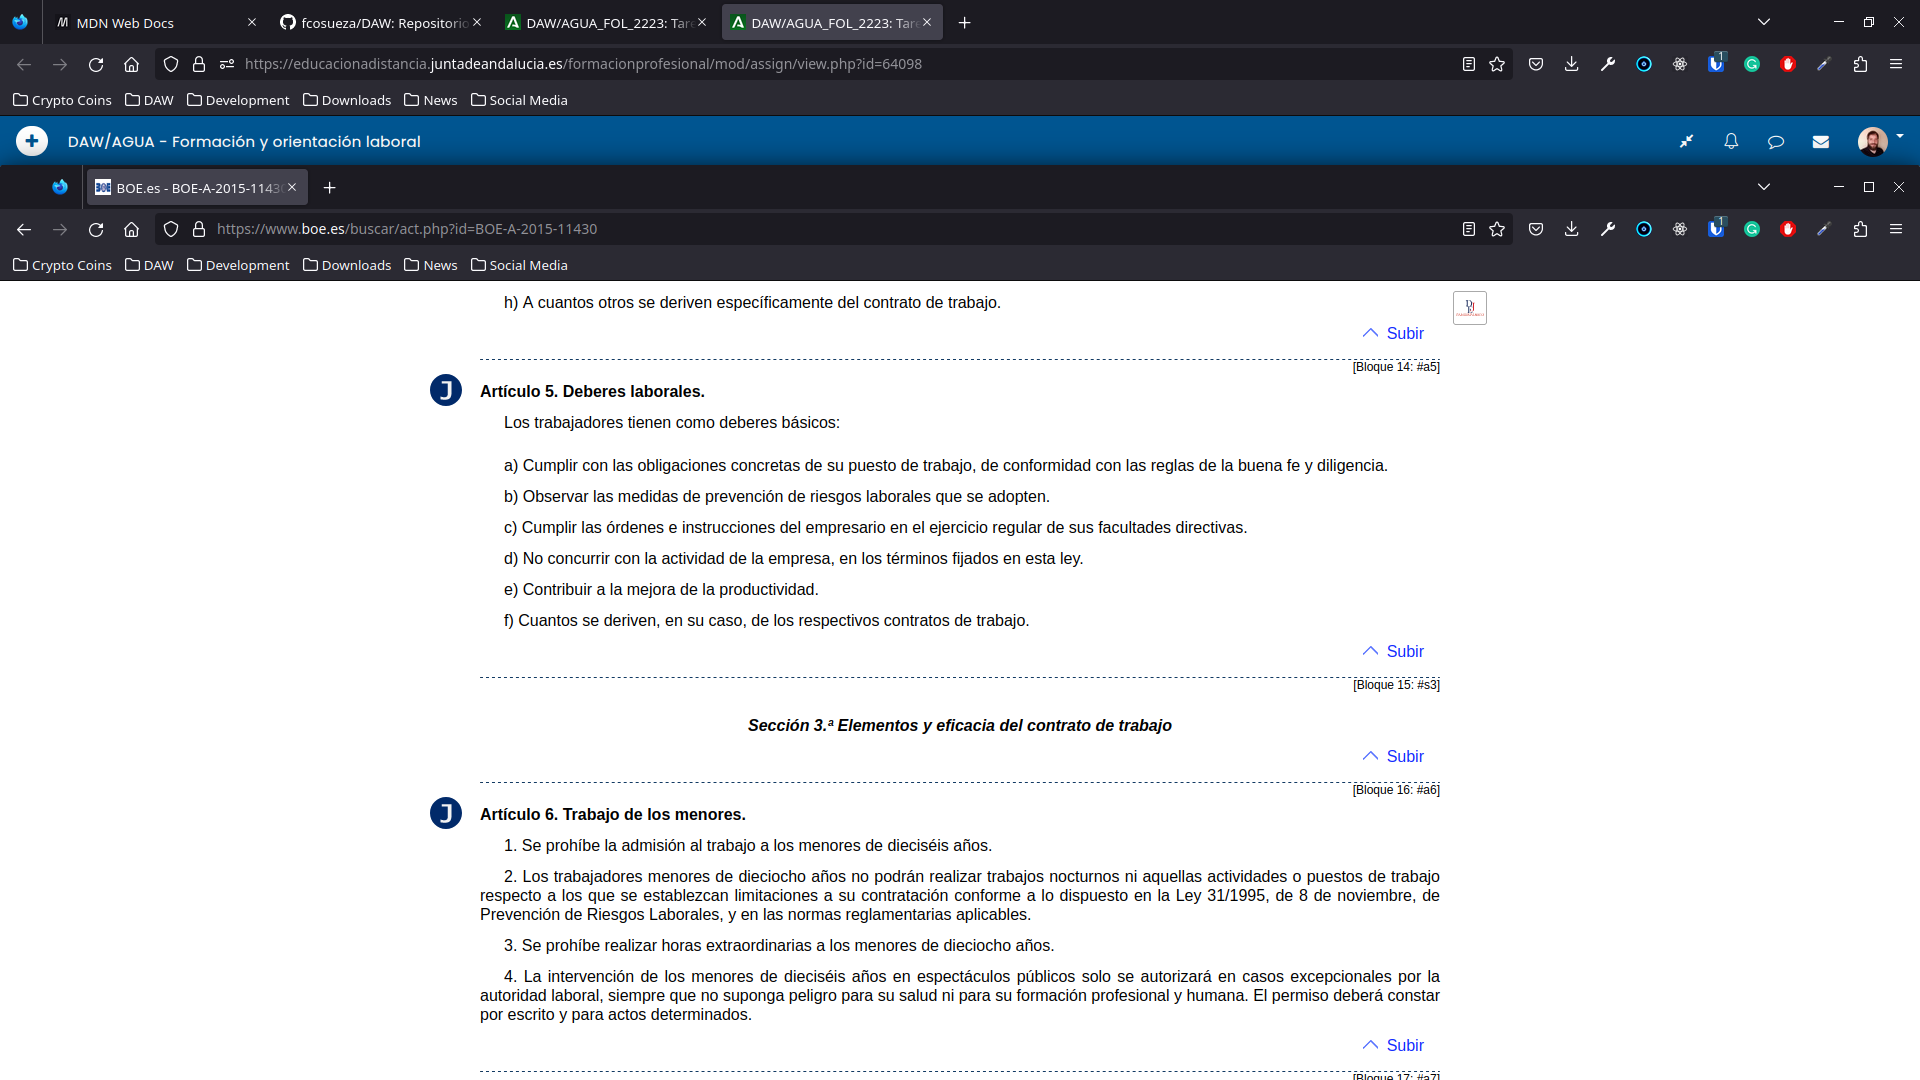
\includegraphics[scale=0.24]{ET-deber.png}
            \caption{Artículo 5 del Estatuto de los Trabajadores}
        \end{figure}

        \item En este apartado hemos escogido el \textbf{artículo 35} de la Constitución Española donde se establece lo siguiente en su punto primero:

        ``Todos los españoles tienen el deber de trabajar y el derecho al trabajo, a la libre elección de profesión u oficio, a la promoción a través del trabajo y a una remuneración suficiente para satisfacer sus necesidades y las de su familia, sin que en ningún caso pueda hacerse discriminación por razón de sexo.'' \cite{const}

        Como dice este punto, es un \textbf{deber} de todos los españoles trabajar, así como un derecho, aunque relativo al deber, entiendo, que se establece para que todos los españoles deban contribuir a la mejora y sustento del país.

        En la siguiente figura se muestra la captura de este artículo:

                \begin{figure}[ht]
            \centering
            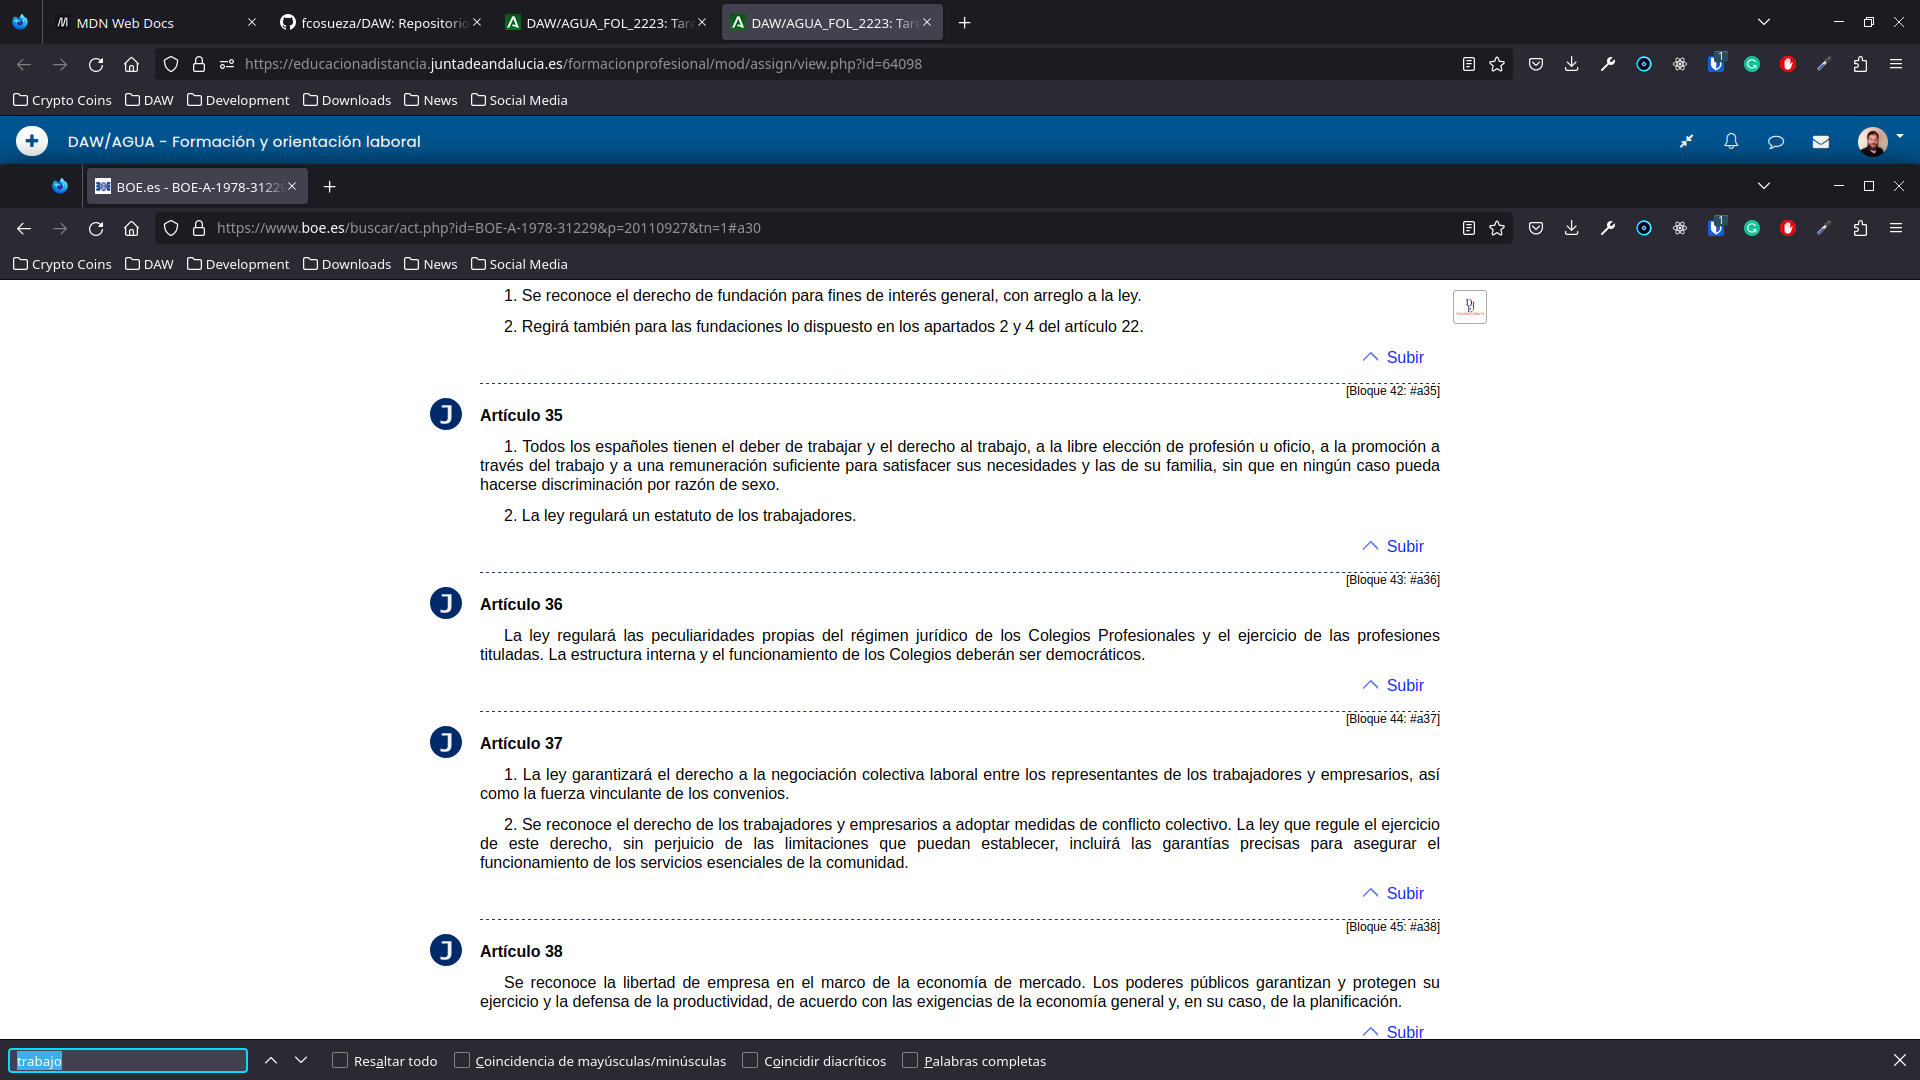
\includegraphics[scale=0.24]{CE-deber.png}
            \caption{Artículo 35 de la Constitución Española}
        \end{figure}
    \end{enumerate}

    \item Caso práctico: Un trabajador incumple uno o varios de sus deberes laborales.
    \begin{enumerate}
        \item Según establece el \textbf{artículo 58} del \textbf{Estatuto de los Trabajadores}, los trabajadores podrán ser sancionados por la dirección de las empresas en caso de incumplimientos laborales, aunque hay que tener en cuenta, que las faltas no deberán de haber prescrito.

        \item Las sanciones y los tipos de faltas (leves, graves y muy graves) se establecen en los convenios colectivos, en el caso de los programadores, en el \href{https://www.boe.es/diario_boe/txt.php?id=BOE-A-2019-14977}{ Convenio colectivo del sector de empresas de ingeniería y oficinas de estudios técnicos.}

        \item Según el \textbf{apartado 3} del \textbf{artículo 58} del \textbf{Estatuto de los Trabajadores}, las sanciones \textbf{nunca} podrán consistir en la \textbf{reducción de los periodos de vacaciones} o cualquier otra minoración de los derechos de descanso del trabajado o \textbf{multa de haber} \cite{rd2015}, consistiendo esta última en la reducción del salario del trabajador.
    \end{enumerate}
\end{enumerate}


\section{Actividad 4}

\subsection{Enunciado}
\textbf{Supuesto práctico:}

AguaCiClo es una empresa lider en instalaciones y servicios informáticos en la provincia de Almería necesita cubrir diferentes puestos. En los supuestos siguientes que se plantean y siempre que sean relaciones laborales, indica el tipo de contrato adecuado y las características esenciales que definen la modalidad.

\begin{enumerate}[label=(\alph*)]
    \item Un puesto de programador, siendo el perfil un titulado en un CFGS de la familia de informática y comunicaciones.
    \item Durante la campaña de navidad 2022/23 se contratará a un operador de ordenador con el fin de reforzar la plantilla al existir un volumen mayor de actividad.
    \item Un puesto de analista a jornada completa cuya titular está desempeñando funciones de representación de los trabajadores en un sindicato.
    \item Con el fin de implementar un programa informático se quiere contratar temporalmente a una empresa para realizar la aplicación hasta su puesta en marcha.
\end{enumerate}

\subsection{Respuesta}

Según los requisitos de los puestos de trabajo enumerados, los \textbf{contratos más apropiados} serán los siguientes:

\begin{enumerate}[label=(\alph*)]
    \item En caso de un programador titulado, el contrato de trabajo más adecuado será un \textbf{contrato de duración indefinida ordinario}, ya que se pretende cubrir un puesto que por norma general va a tener larga duración en el tiempo.

    \textbf{La principal característica} de este tipo de contrato es que \textbf{no se define} una duración determinada para el contrato, por lo que su duración es indefinida. Estos contratos pueden ser a \textbf{jornada completa} o \textbf{parcial}.

    \item En este caso, el contrato que mejor se adaptaría a la situación sería un \textbf{contrato fijo discontinuo}, ya que nos encontramos ante un trabajo de temporada, porque este aumento de la actividad se producirá en todas las campañas de navidad.

    Este contrato alterna períodos de trabajo y no trabajo en al empresa, ya sea por trabajos estacionales o de temporada. Es el tipo de contrato más asociado con las ETTs y sus principales características son:

    \begin{itemize}
        \item Siguen un orden de llamamiento establecido por convenio.
        \item Se computa como antigüedad el tiempo o periodo inactivo entre llamamientos.
    \end{itemize}

    \item En este caso, teniendo en cuenta que la trabajadora hace las funciones de \textbf{enlace sindical}, el contrato más apropiado sería el de \textbf{contrato de duración indefinida ordinario}, ya que una de las condiciones para poder realizar la función de enlace sindical es la de tener, al menos, \textbf{6 meses de antigüedad} en la empresa, como establece el \textbf{artículo 69} del \textbf{Estatuto de los Trabajadores}, por lo que no sería posible realizar un contrato de duración determinada.

    \item Este caso es un poco peculiar. Aunque se nos indica en el enunciado que es un trabajo ``\textbf{temporal}'', no sabemos exactamente la duración de ésta. Podríamos pensar en un contrato de duración determinada, pero este caso en concreto entraría dentro de la categoría de \textbf{contrato por circunstancias de la producción previsible}, por lo que estaríamos limitados a 90 días, que además, no pueden ser continuos, por lo que \textbf{este tipo de contrato no nos serviría}.

    Con la antigua legislación, esto sería un \textbf{contrato por obra y servicio} de manual, pero esta modalidad de contrato ha desaparecido con la \textbf{reforma laboral de 2022}, por lo que teniendo en cuenta todas las circunstancias, el contrato más adecuado para este caso sería un \textbf{contrato de duración indefinida ordinario.}
\end{enumerate}

\section{Actividad 5}
\subsection{Enunciado}
Respecto a las medidas de conciliación elige aquella que consideres, valora.


\subsection{Respuesta}
Una de las medidas que más favorecen es la del \textbf{teletrabajo} o \textbf{trabajo a distancia}, introducida como medida de conciliación familiar en el \href{https://www.boe.es/buscar/act.php?id=BOE-A-2019-3244&p=20190307&tn=1#a1}{Real Decreto-ley 6/2019, de 1 de marzo} de medidas urgentes para garantía de la igualdad de trato y de oportunidades entre mujeres y hombres en el empleo y la ocupación.

Es una medida que me parece muy apropiada, ya que favorece en gran medida la conciliación familiar, siendo mi opinión personal, que es una de las que más lo favorecen. El hecho de poder desarrollar el trabajo desde casa hace que podamos estar muchas más horas con la familia en nuestro hogar, algo, que según algunos estudios, también aumenta la productividad. Por otra parte, es una medida a la que no todos los trabajadores pueden acogerse, ya que sus empleos son necesariamente presenciales y sería imposible solicitar esta medida.

\section{Actividad 6}
\subsection{Enunciado}
Un trabajador con la categoría profesional de programador informático, grupo 2 de cotización a la Seguridad Social, presta sus servicios en la empresa ``AguaCiClo'' desde el 1/08/19 mediante contrato indefinido a jornada completa. Las retribuciones pactadas, de percepción mensual, son las siguientes:
\begin{itemize}
    \item Salario Base: 1100 €
    \item Complemento de jefatura: 80 €
    \item Complemento antiguedad: 50 € por trienio
    \item Horas extraordinarias realizadas ese mes: 80 €
    \item Tiene derecho a 2 Pagas Extraordinarias, a percibir en Junio y Diciembre, de salario base más complemento de jefatura cada una de ellas. Cuando lleguen los meses correspondientes cobrará las pagas íntegras.
    \item IRPF 10\%
\end{itemize}

Calcula y justifica los siguientes conceptos de un mes normal que no sea Junio o Diciembre.

\begin{itemize}
    \item Remuneración mensual (salario bruto)
    \item Base de Cotización por Contingencias Comunes
    \item Base de cotización por Contingencias Profesionales.
    \item Salario líquido a percibir (salario neto).
\end{itemize}

\subsection{Respuesta}

\begin{itemize}
    \item En primer lugar vamos a calcular el \textbf{salario bruto} del trabajador, que es el total que el empresario le paga al trabajador, es decir, el \textbf{total devengado}, sin aplicar ninguna deducción.

    Así deberá sumarse la \textbf{base de cotización}, más todos los \textbf{complementos salariales} y \textbf{no salariales} y las \textbf{horas extraordinarias}.

        \begin{figure}[H]

        \vspace{3ex}
        \centering

        \setlength{\tabcolsep}{10pt}
        \renewcommand{\arraystretch}{1.4}

        \begin{tabular}{| l | r |}
            \hline
            \textbf{Concepto}  & \textbf{Cantidad} \\ \hline
            \centering - Base de Cotización & 1100€  \\ \hline
            \centering - Complemento de Jefatura & 80€  \\ \hline
            \centering - Complemento de Antigüedad & 50€  \\ \hline
            \centering - Horas Extras & 80€  \\ \hline
            \centering \textbf{TOTAL} &  \textbf{1310€} \\ \hline
        \end{tabular}
        \caption{Cálculo de Salario Bruto}
    \end{figure}

    \item A continuación vamos a calcular la \textbf{base de cotización por contingencias comunes}. Este cálculo es similar al del salario bruto con un par de diferencias, estas son que \textbf{no se incluyen las horas extras} y en cambio, \textbf{si se incluyen} las  \textbf{pagas extras prorrateadas}, por lo que el cálculo quedaría como vemos en la siguiente tabla:

    \begin{figure}[H]

        \vspace{3ex}
        \centering

        \setlength{\tabcolsep}{10pt}
        \renewcommand{\arraystretch}{1.4}

        \begin{tabular}{| l | r |}
            \hline
            \textbf{Concepto}  & \textbf{Cantidad} \\ \hline
            \centering - Base de Cotización & 1100€  \\ \hline
            \centering - Complemento de Jefatura & 80€  \\ \hline
            \centering - Complemento de Antigüedad & 50€  \\ \hline
            \centering - Pagas extras prorrateadas &  196,6€ \\ \hline
            \centering \textbf{TOTAL} &  \textbf{1426,6€} \\ \hline
        \end{tabular}
        \caption{Base de cotización por contingencias comunes}
    \end{figure}


    \item Ahora vamos a calcular la \textbf{base de cotización por contingencias profesionales}, que se obtiene sumando a la cotización por contingencias comunes las horas extras, en caso de que las hubiera.

     \begin{figure}[H]

        \vspace{3ex}
        \centering

        \setlength{\tabcolsep}{10pt}
        \renewcommand{\arraystretch}{1.4}

        \begin{tabular}{| l | r |}
            \hline
            \textbf{Concepto}  & \textbf{Cantidad} \\ \hline
            \centering - Base de Cotización & 1100€  \\ \hline
            \centering - Complemento de Jefatura & 80€  \\ \hline
            \centering - Complemento de Antigüedad & 50€  \\ \hline
            \centering - Pagas extras prorrateadas &  196,6€ \\ \hline
            \centering - Horas Extras & 80€  \\ \hline
            \centering \textbf{TOTAL} &  \textbf{1506,6€} \\ \hline
        \end{tabular}
        \caption{Base de cotización por contingencias profesionales}
    \end{figure}

    \item Por último, vamos a calcular el salario neto que recibe el trabajador. Para ello tenemos que aplicar un conjunto de deducciones sobre el \textbf{salario bruto}, la \textbf{BCCC}, la \textbf{BCCF} y la \textbf{BHE} (base de horas extras). Las deducciones que debemos aplicar a cada una de las bases son las siguientes:

    \begin{itemize}
        \item \textbf{Salario Bruto}: sobre el salario bruto hay que aplicar las retenciones del \textbf{IRPF}, que en este caso es de un 10\%.
        \item \textbf{Base de Cotización por Contingencias Comunes}: sobre esta base hay que aplicar una deducción del \textbf{tipo de cotización}, que en este caso es del 4,7\%.
        \item \textbf{Base de Cotización por Contingencias Profesionales}: de esta base hay que deducir la \textbf{cotización por desempleo}, que es de un 1,55\% y la de \textbf{FP}, que es un 0,10\%.
        \item \textbf{Base Horas Extras}: por último, hay que aplicar la \textbf{deducción a las horas extras}, como no se nos indica si son por fuerza mayor o no, entenderemos que no son por fuerza mayor, por lo que aplicaremos un tipo del 4.7\%.
    \end{itemize}

    En la siguiente tabla, se muestra el cálculo de todas las deducciones:

      \begin{figure}[H]

        \vspace{3ex}
        \centering

        \setlength{\tabcolsep}{10pt}
        \renewcommand{\arraystretch}{1.4}

        \begin{tabular}{| l | r |}
            \hline
            \textbf{Deducción}  & \textbf{Cantidad} \\ \hline
            \centering - IRPF (10\%) &  131€ \\ \hline
            \centering - Contingencias Comunes (4.7\%) & 67€ \\ \hline
            \centering - Desempleo (1,55\%) & 23,3€  \\ \hline
            \centering - FP (0,10\%)& 1,5€ \\ \hline
            \centering - BHE (4,7\%) & 3,76€  \\ \hline
            \centering \textbf{TOTAL} &  \textbf{226,56€} \\ \hline
        \end{tabular}
        \caption{Cálculo de las deducciones}
    \end{figure}

    Una vez que hemos calculado todas las deducciones, ya solo nos queda restarlo al salario bruto o total devengado y obtendremos en salario líquido a percibir, que en nuestro caso sería:

       \vspace{3ex}
       \centering\textbf{Salario Líquido a Percibir} = 1310€ - 226,56€ = \textbf{1083,44€}

\end{itemize}

\section{Actividad 7}
\begin{enumerate}
    \item Responde a los siguientes cuestiones:
    \begin{enumerate}
        \item Diferencia entre suspensión, modificación y extinción de la relación laboral, explicando brevemente los diferentes conceptos y además añade un ejemplo de cada una de ellos.
        \item Respecto a las modificaciones geográficas:
        \begin{enumerate}
            \item Cita los tipos.
            \item Diferencia una de la otra.
            \item Ejemplifica cada una de ella.
        \end{enumerate}
    \end{enumerate}

    \item \textbf{Caso Práctico}:

    La empresa ``AguaCiClo'' comunica a su trabajadora Paula Galdano que el día 30 de octubre 2022 termina su contrato de trabajo por tiempo indefinido al aplicarle un despido objetivo por cuestiones económicas. La comunicación se la realiza verbalmente el encargado de RRHH.  El despido se hará efectivo el día 31 de octubre de 2022, y poniendo a disposición del trabajador el finiquito.

    \begin{enumerate}
        \item Detalla lo/s incumplimientos por parte de la empresa si los hubiera.
        \item ¿Crees que  le corresponde a Paula recibir indemnización, además del finiquito, el día que se hace efectivo el despido?
        \item Si quiere reclamar Paula, ¿puede hacerlo poniendo la demanda judicial directamente o es necesario algún procedimiento previo en plazo? Justifica la respuesta
        \item Una vez celebrado juicio, el juez declara el despido objetivo como improcedente, ¿qué opciones tiene la empresa para solventar la situación tras la sentencia judicial?
    \end{enumerate}
\end{enumerate}

\subsection{Respuesta}
\begin{enumerate}
    \item Responde a los siguientes cuestiones:
    \begin{enumerate}
    \item En este punto vamos a ver la diferencias que existe entre la modificación, suspensión y extinción de un contrato laboral.

        \begin{itemize}
            \item \textbf{Suspensión del contrato}: una suspensión del contrato implica un \textbf{cese en las obligaciones} de \textbf{trabajar} y \textbf{remunerar el trabajo} por alguna de las causas previstas en la ley o el convenio colectivo. Una vez cesada la causa de la suspensión, la relación laboral se vuelve a reanudar. Dependiendo de la causa que motive la suspensión, la suspensión puede ser \textbf{con reserva del puesto de trabajo} o \textbf{sin reserva del puesto de trabajo}.

            \textbf{Un ejemplo} de suspensión sería la que sucede cuando se convoca una \textbf{huelga o un cierre patronal}, que es una causa de suspensión colectiva

            \item \textbf{Modificación del contrato}: una \textbf{modificación del contrato} consiste en la \textbf{alteración} de las \textbf{condiciones} de la relación laboral, que puede suceder por diferentes motivos. Además, los empresario puede modificar las condiciones dentro de unos límites y siempre respetando los derechos del trabajador.

            \textbf{Un ejemplo} de modificación del contrato podría darse por un \textbf{cambio en el convenio} en el que se aumente, por ejemplo, el salario mínimo del puesto que desempeña el trabajador, por lo que habría que actualizarlo en el contrato.

            \item \textbf{Extinción del contrato de trabajo}: la extinción del contrato implica el cese definitivo de los efectos del contrato de trabajo. Siempre debe de haber una causa para la extinción del contrato. Dependiendo de ésta causa, el trabajador tendrá derecho a indemnización y desempleo, o no.

            \textbf{Un ejemplo} de extinción se daría cuando las partes, \textbf{de mutuo acuerdo}, deciden la extinción del contrato, por ejemplo, porque no quieren seguir con la relación laboral por desavenencias personales entre trabajadores y empresario. En este caso, el trabajador no tendría derecho ni a indemnización ni a prestaciones por desempleo.
        \end{itemize}

    \item Las \textbf{modificaciones geográficas} se producen cuando por diferentes razones, como económicas, técnicas, organizativas o  de producción, la empresa ordena un \textbf{cambio de lugar de trabajo}, lo que implicaría también un cambio de residencia del trabajador.

    Dependiendo de la duración y el número de trabajadores afectados, las modificaciones geográficas pueden ser:


    \begin{itemize}
        \item Según la \textbf{duración}:
        \begin{itemize}
            \item \textbf{Traslado}: si la \textbf{duración es mayor} de 12 meses en un período de 3 años.
            \item \textbf{Desplazamiento}: si la \textbf{duración es menor}	de 12 meses en un período de 3 años.
        \end{itemize}
        \item Según el \textbf{numero de trabajadores}:
        \begin{itemize}
         \item \textbf{Colectivo}: se considera que un traslado o desplazamiento es colectivo cuando se traslada a todos los trabajadores de una empresa, o sí no se traslada a todos, cuando se realiza con los siguientes trabajadores \cite{mites}:
        \begin{itemize}
            \item Diez trabajadores, en las empresas que ocupen menos de cien trabajadores.
            \item El 10 por 100 del número de trabajadores de la empresa que ocupe entre cien y trescientos trabajadores.
            \item Treinta trabajadores en las empresas que ocupen más de trescientos trabajadores.
        \end{itemize}
        \item \textbf{Individual}: un traslado o desplazamiento se considera individual cuando se realiza sobre un número de trabajadores inferior al indicado en el punto anterior.
        \end{itemize}
    \end{itemize}

    A continuación se enumeran algunos ejemplos con los diferentes tipos combinados:

    \begin{itemize}
        \item \textbf{Desplazamiento Individual}: si por ejemplo una cuadrilla de albañilería, menos de 10 trabajadores, le hicieran desplazarse a otra provincia para la realización de una obra, con un periodo de ejecución de 6 meses.

        \item \textbf{Desplazamiento Colectivo}: si una empresa con 25 trabajadores, dedicada a la evaluación de riesgos laborales debe desplazar a 15  trabajadores a una provincia colindante para la supervisión de la construcción de un estadio de fútbol.

        \item \textbf{Traslado Individual}: si a un comercial de ventas le comunicarán que han abierto una nueva sucursal en otra comunidad autónoma y tuviera que ejercer su trabajo allí de forma indefinida.

        \item \textbf{Traslado Colectivo}: en el caso de que una empresa, por ejemplo, traslade su única factoría de producción a otra comunidad autónoma, teniendo todos los trabajadores que moverse a la nueva ubicación.
    \end{itemize}
    \end{enumerate}


    \item \textbf{Caso Práctico}:

    \begin{enumerate}
        \item La \textbf{empresa a incumplido} la forma de comunicación del despido a la trabajadora. Esta debe realizarse \textbf{por escrito}, no siendo válida en ninguna circunstancia la comunicación verbal. Tampoco se especifica en que momento se le ha realizado la comunicación, por lo que no sabemos si se ha cumplido con el plazo de preaviso  de 15 días.

        \item Sí. En los \textbf{despidos por causas objetivas}, en el caso de que sean procedentes, a Paula le correspondería una indemnización de \textbf{20 días por año trabajado}, hasta un máximo de 12 mensualidades.

        \item No, para poder demandar primero debe de haber un acto de \textbf{conciliación previa}, requisito obligatorio antes de una demanda en el Juzgado de lo Social, y con el que se pretende llegar a un acuerdo por ambas partes, antes del proceso judicial.

        \item La empresa, una vez declarado el despido improcedente, tiene un plazo de 5 días para:
        \begin{itemize}
            \item \textbf{Readmitir} a la trabajadora en su puesto. En este caso la trabajadora tendrá derecho a los salarios de tramitación, es decir, a los salarios que ha dejado de percibir.
            \item \textbf{Extinguir el contrato} con la trabajadora, con una indemnización de 33 días por año trabajado con un máximo de 24 mensualidades.
        \end{itemize}

        También quedará siempre la opción de poner un recurso en los órganos judiciales superiores, aunque dependiendo del caso esto no siempre es posible.
    \end{enumerate}
\end{enumerate}

% Bibliography

\newpage
\bibliography{citas}
\bibliographystyle{unsrt}

\end{document}